\documentclass[serif]{beamer}

 %\usepackage{eulervm}
 %\usepackage{arev}
 %\usepackage{mathpazo}
 %\usepackage[charter]{mathdesign}
 \usepackage{charter}
 \usepackage{color}
 \usepackage{enumerate}
 \usepackage{amsfonts,amssymb}
 \usepackage{tikz}

 \beamertemplatenavigationsymbolsempty

 \definecolor{cambridgeblue}{RGB}{163,193,173}
 \definecolor{altrosa}{RGB}{201,119,153}
 \definecolor{cambridgegreen}{RGB}{87,116,97}
 \definecolor{dorian}{RGB}{70,70,70}
 \setbeamercolor{frametitle}{fg=cambridgeblue}
 \setbeamercolor{title}{fg=cambridgeblue}
 \setbeamercolor{itemize item}{fg=cambridgegreen}
 \setbeamercolor{enumerate item}{fg=cambridgegreen}
 \setbeamercolor{block title}{fg=cambridgegreen}
 \setbeamercolor{section in toc}{fg=cambridgegreen}
 \setbeamercolor{alerted text}{fg=altrosa}
 \setbeamercolor{normal text}{fg=dorian}
 
 \addtobeamertemplate{frametitle}{\vskip+100pt}{}
 \setbeamertemplate{frametitle}[default][left]
 \setbeamerfont{frametitle}{size = \huge}
 \setbeamerfont{frametitle}{series = \bfseries}
 \setbeamerfont{title}{size = \huge}
 \setbeamerfont{title}{series = \bfseries}
 \setbeamertemplate{footline}[frame number]
 \setbeamertemplate{caption}{\raggedright\insertcaption\par}
 
 \renewenvironment{quote}
  {\begin{trivlist} \setlength\leftskip{0cm} \setlength\rightskip{0pt}
   \item\relax}
  {\end{trivlist}}

\usepackage{rotating,accsupp,mathtools} % for \rotatebox for riota
 
    \newcommand{\tto}{\Rightarrow}
    \newcommand{\ffrom}{\Leftarrow}
    \renewcommand{\iff}{\leftrightarrow}
    \newcommand{\among}{\preccurlyeq}
    
  \newcommand{\defeq}{\vcentcolon= \ }
  \newcommand{\eqdef}{=\vcentcolon}
    
    \newcommand{\disq}[1]{$\ulcorner {#1} \urcorner$}
    % NB could also use \textopencorner {#1}\textcorner without mathmode    
    
    \newcommand*{\riota}{\mathord{%
    \BeginAccSupp{method=hex,unicode,ActualText=2129}%
    \text{\raisebox{\depth}{\rotatebox{180}{\(\upiota\)}}}%
    \EndAccSupp{}}}

%\setbeameroption{show notes} %un-comment to see the notes
%\setbeamertemplate{note page}[plain] %for printing

\title[title]
{Superplural~Logic}
\subtitle{MoL~Thesis~Defence}
\author{Eileen~Wagner}
\AtBeginSection[]{\begin{frame}\frametitle{Outline}\tableofcontents[currentsection]\end{frame}}
\AtBeginSubsection[]{\begin{frame}\frametitle{Outline}\tableofcontents[currentsubsection]\end{frame}}
\date{20/11/2015}

\begin{document}

\frame{\titlepage}

\begin{frame}
\frametitle{}

plural logic?
\note{crash course...}

\end{frame}

\begin{frame}
\frametitle{Plural logic}

FOL \pause + $xx, yy, \dots$ \pause + $\among$
\pause

$\exists xx ~ \mathit{Apple}(xx)$

\pause
\begin{block}{collective predication}\pause
\begin{enumerate}[<+->]
  \item[a] `Russell and Whitehead were logicians.'
  \item[a*] `Russell was a logician and Whitehead was a logician.'
  \item[b] `Russell and Whitehead co-authored \emph{Principia Mathematica}.'
  \item[b*]  `Russell co-authored \emph{Principia Mathematica} and Whitehead co-authored \emph{Principia Mathematica}.'
  \end{enumerate}
\end{block}
\pause
$\{ \mathit{Russell}, \mathit{Whitehead}\}$ ?
\end{frame}

\begin{frame}
\frametitle{Singularisation}

Problem with \alert{singular surrogates}
\medskip

\begin{itemize}
  \item changing the subject
  \item Russelian paradox
\end{itemize}
%\onslide<2>{$\exists xx (\forall y (y \among xx \to (y = r \lor y = w)) \land \mathit{WrotePrincipia}(xx))$}

\end{frame}

\begin{frame}
\frametitle{Ideology}

\begin{quote}
  `\dots abandoning the fetish for the singular that pervades contemporary decadent Western ontology.'
\end{quote}
{\raggedleft\footnotesize Richard Sharvy, 1980\par}
\end{frame}

\begin{frame}
\frametitle{Outline}
\tableofcontents
\end{frame}

\section{What are superplurals?}

\begin{frame}
\frametitle{Superplurals}

\begin{itemize}
  \item `Russell and Whitehead, and Hilbert and Bernays'
  \item `the Boswell Sisters and the Mills Brothers'
  \item `the twin primes'
\end{itemize}
\note{again, assuming you think the B sisters is a plural term}
\end{frame}

\begin{frame}
\frametitle{Supersuperplurals}
\begin{itemize}
  \item `the Yankees and the Red Sox, and the Giants and the Braves'
\end{itemize}
\note{championship series}
\end{frame}

\begin{frame}
\frametitle{Literature}

Hazen (1997), Linnebo (2003), Uzquiano (2004), McKay (2006), Rayo (2006), Linnebo \& Nicolas (2008), Florio (2010), Oliver \& Smiley (2013), Ben-Yami (2013), Rieppel (2015), Simons (1982, forthcoming)

\note{aim of the thesis: to gather arguments, unified account, discussion}

\end{frame}

\begin{frame}
\frametitle{Notation}

\small{
\begin{table}[htpb]
\centering
\begin{tabular}{l| c c}
& plural variables & superplural variables \\
\hline
Simons (1982)  & $h, k, l; u,v,w$  &         \\
Burgess \& Rosen (1997) & $xx, yy, zz$    &           \\
Linnebo (2003) & $xx, yy, zz$    &           \\
Rayo (2006)   & $xx, yy, zz$    & $xxx, yyy, zzz$   \\
McKay (2006)  & $X, Y, Z$     & $XX, YY, ZZ$    \\
Yi (2006)       & $xs, ys, zs$    &           \\
Nicolas (2008)   & $xs, ys, zs$    & $xss, yss, zss$   \\
Oliver \& Smiley (2013)  & $\mathbf{x,y,z}$  & $\mathbf{x^2,y^2,z^2}$  \\
\end{tabular}
\caption{previous notations for plural and superplural terms}\label{tab:terms}
\end{table}
}
\end{frame}

\begin{frame}
\frametitle{Notation}

\small{
\begin{table}[htpb]
\centering
\begin{tabular}{l| c l}
& predicate & reading \\
\hline
Simons (1982)  & $\in$   & is or is among\\
              & $\rotatebox{90}{\(\pitchfork\)}$ & is/are or is/are among\\
Burgess \& Rosen (1997)  & $= =$   & is or is among      \\
Linnebo (2003) & $\prec$ & is among          \\
Burgess (2004)   &$\alpha$ & is or is among      \\
Rayo (2006)     & $\prec$   & is or is among      \\
              & $\precsim$  & is/are or is/are among  \\
McKay (2006)   & K     & is or is among      \\
              & A     & is/are or is/are among  \\
Yi (2006)        & H     & is or is among      \\
              & $\sqsubseteq$   & is/are or is/are among  \\
Nicolas (2008)  & $\angle$  & is/are or is/are among  \\
Oliver \& Smiley (2013)  & $\among$  & is/are or is/are among  \\
Florio (2014) & $\prec$ & is among          \\
Simons (2016)  & $\eta$  & is one of
\end{tabular}
\caption{previous notations for the inclusion predicate}
\end{table}
}
\end{frame}

\section{Why superplurals?}

\begin{frame}
\frametitle{Why superplurals?}
\begin{itemize}[<+->]
  \item occurrence in natural language
  \item ontological innocence
\end{itemize}
\end{frame}

\begin{frame}
\frametitle{}
\begin{center}
\includegraphics[width=\textwidth,height=0.8\textheight,keepaspectratio]{quine.jpg}
\end{center}
\end{frame}

\section{Why not?}

\begin{frame}
\frametitle{Two objections}

\only<1>{\alert{Intelligibility}\\
higher-level plural quantification is unintelligible}
\only<2>{\alert{Naturalness}\\
there are no genuine examples of superplurals in natural language}
\note{these two reasons have attracted two kinds of criticism}
\end{frame}


\subsection{Naturalness}

\begin{frame}
\frametitle{Examples}
\begin{itemize}
  \item `Russell and Whitehead, and Hilbert and Bernays wrote multivolume logic books together.'
  \item `The Boswell Sisters and the Mills Brothers gave a joint concert.'
  \item `The twin primes are infinite in number.'
\end{itemize}
\end{frame}

\begin{frame}
\frametitle{Strategies for paraphrase}
\begin{itemize}
  \item partial singularisation (groups)
  \item conjunctive analysis (distributive)
  \item ordinary plural analysis (lists)
  \item multigrade predicates (superplurals)
\end{itemize}
\end{frame}

\begin{frame}
\frametitle{\dots and why they fail}

\emph{The boys and the girls played against each other.}

\end{frame}

\begin{frame}
\frametitle{Finnish}
{\small
\begin{figure}[htb]
\centering
\begin{tabular}{l l l}
VALUE & SINGULAR & PLURAL \\
1 & yksi & yhdet\\
2 & kaksi & kahdet\\
3 & kolme & kolmet\\
4 & nelj{\"a} & nelj{\"a}t\\
5 & viisi & viidet\\
6 & kuusi & kuudet\\
7 & seitsem{\"a}n & seitsem{\"a}t\\
8 & kahdeksan & kahdeksat\\
9 & yhdeksa{\"a}n & yhdeks{\"a}t\\
10 & kymmenen & kymmenet\\
&&\\
pair, couple & pari & parit\\
a few & muutama & muutamat\\
many & moni & monet\\
several & usea & useat\\
a few, not many & harva & harvat
\end{tabular}
\end{figure}
}
\end{frame}

\subsection{Intelligibility}

\begin{frame}
\frametitle{Intelligibility}

\begin{itemize}[<+->]
  \item collapse \note{many people as well, just has a little more structure... > ordinary plural logic}
  \item collapse vs. singularisation \note{I think it's worse!}
\end{itemize}
\end{frame}

\begin{frame}
\frametitle{Iteration}
\begin{quote}
   A natural question that arises is whether the step from the singular to the plural can be iterated. Are there terms that stand to ordinary plural terms the way ordinary plural terms stand to singular terms? Let's call such terms superplurals. A superplural term would thus, loosely speaking, refer to several `pluralities' at once, much as an ordinary plural term refers to several objects at once.
\end{quote}
{\raggedleft\footnotesize Linnebo \& Nicolas, 2008, p. 186 \par}
\end{frame}

\begin{frame}
\frametitle{Which picture?}

\begin{figure}[ht]
\centering
{
    \begin{tikzpicture}
    \tikzstyle{level 1}=[level distance=15mm, sibling distance=30mm]
    \tikzstyle{level 2}=[level distance=15mm, sibling distance=15mm] 
    \node {sp}
    child {node {p}
    child {node {$\bullet$}}
    child {node {$\bullet$}}
    }
    child {node {p}
      child {node {$\bullet$}}
      child {node {$\bullet$}}
    };
\end{tikzpicture}
}
\caption{superplural reference\label{fig:cover}}
\end{figure}
\pause
\alert{singularisation?}
\end{frame}

\begin{frame}
\frametitle{Which picture?}

\begin{figure}[hp]
\centering
{
    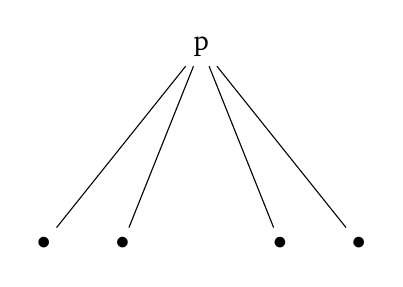
\begin{tikzpicture}
    \tikzstyle{level 1}=[level distance=25mm, sibling distance=10mm]
    \node {p}
    child {node {$\bullet$}}
    child {node {$\bullet$}}
    child {node {} edge from parent[draw=none]}
    child {node {$\bullet$}}
    child {node {$\bullet$}
    };
\end{tikzpicture}
}
\caption{plural reference + X\label{fig:art}}
\end{figure}
\pause
\alert{collapse?}
\end{frame}

\note{1 smuggles in structure. how to understand first picture. 2 mistake is sp reference is its own thing... that's why iteration doesn't work!}

\section{Alternative accounts}   

\begin{frame}
\frametitle{Cover semantics}

\begin{equation*}
  \mathcal{D}(F) = \lambda x [\forall y (y \in C_x \to F(y))]
\end{equation*}
\only<2-3>{Russell and Whitehead, and Hilbert and Bernays were logicians.}

\only<3>{$\forall y (y \in \{\text{ \{Russell\}, \{Whitehead\}, \{Hilbert\}, \{Bernays\}}\}\to \mathit{Logician}(y))$}

\onslide<4->{Russell and Whitehead, and Hilbert and Bernays wrote multivolume logic books together.}

\only<5>{$\forall y (y \in \{\{\text{Russell, Whitehead}\}, \{\text{Hilbert, Bernays}\}\} \to \mathit{WroteLogicBook}(y)) $}

\end{frame}

\begin{frame}
\frametitle{Two hierarhies}

\begin{figure}[htbp]
\begin{center}
    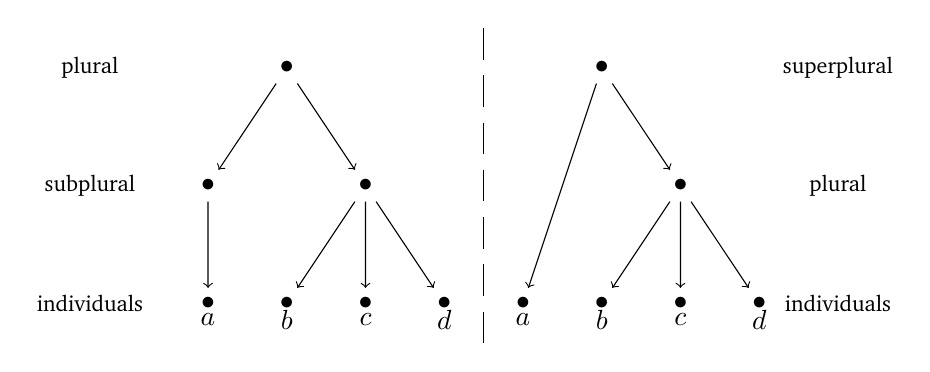
\begin{tikzpicture}
    [edge from parent/.style={draw,-to}]
    \tikzstyle{level 1}=[level distance=15mm, sibling distance=20mm]
    \tikzstyle{level 2}=[level distance=15mm, sibling distance=10mm] 
    \node  (SUB) at (-2.5,0) {$\bullet$}
    child {node {$\bullet$}
    child {node (SUBa){$\bullet$}}
    }
    child {node {$\bullet$}
      child {node (SUBb){$\bullet$}}
      child {node (SUBc){$\bullet$}}
      child {node (SUBd){$\bullet$}}
    };
    \node  (SUPER) at (1.5,0) {$\bullet$}
    child {coordinate [edge from parent/.style={draw=none}] {}
    }
    child {node {$\bullet$}
      child {node (SUPERb){$\bullet$}}
      child {node (SUPERc){$\bullet$}}
      child {node (SUPERd){$\bullet$}}
    };
    \draw (0.5,-3) node(SUPERa) {$\bullet$};
    \draw[->] (SUPER) -- (SUPERa);
    \draw (SUBa.south)  node {$a$};
    \draw (SUBb.south)  node {$b$};
    \draw (SUBc.south)  node {$c$};
    \draw (SUBd.south)  node {$d$};
    \draw (SUPERa.south)  node {$a$};
    \draw (SUPERb.south)  node {$b$};
    \draw (SUPERc.south)  node {$c$};
    \draw (SUPERd.south)  node {$d$};
    \draw (-5,0) node(SUBplural) {\footnotesize plural};
    \draw (-5,-1.5) node(SUBsubplural) {\footnotesize subplural};
    \draw (-5,-3) node(SUBind) {\footnotesize individuals};
    \draw (4.5,0) node(SUPERplural) {\footnotesize superplural};
    \draw (4.5,-1.5) node(SUPERsubplural) {\footnotesize plural};
    \draw (4.5,-3) node(SUPERind) {\footnotesize individuals};
    \draw[dash pattern=on 4mm off 2mm] (0,0.5) -- (0,-3.5);
\end{tikzpicture}
\caption{comparing the hierarchies\label{fig:compare}}
\end{center}
\end{figure}
\end{frame}

\begin{frame}
\frametitle{Structure}

\begin{itemize}[<+->]
  \item Accounts differ in how they add structure to reference.
  \item Cover semantics needs a stronger structure, leading to a subplural hierarchy. 
  \item The subplural and the superplural hierarchy are two conceptions of superplural reference.
\end{itemize}

\end{frame}

\section{Innocence}

\begin{frame}
\frametitle{Ontological commitment}

A first-order sentence carries commitment to Fs just in case Fs must be counted amongst the values of the variables in order for the sentence to be true.

\end{frame}

\begin{frame}
\frametitle{Plethological commitment}

A singular or plural first-order sentence carries commitment to Fs just in case Fs must be counted amongst the values of the (singular or plural) variables in order for the sentence to be true.
\end{frame}

\begin{frame}
\frametitle{Higher-level plethological commitment}

An n-level first-order sentence carries commitment to Fs just in case Fs must be counted amongst the values of the n-level variables in order for the sentence to be true.
\note{end of story? not quite...}

\end{frame}

\begin{frame}
\frametitle{The end?}

\onslide<2>{\alert{ontology vs. ideology}}

\end{frame}

% \begin{frame}
% \frametitle{Summary}

% \begin{itemize}[<+->]
%   \item Superplural logic is a perfectly good way to capture higher-level quantification.
%   \item There is a natural way to build a superplural hierarchy.
%   \item Superplural logic has no further ontological commitments.
% \end{itemize}
% \end{frame}

\note{and that was a very quick run-through of my thesis!}

\begin{frame}
\begin{center}
{\huge thank you!}
\end{center}
\end{frame}

\appendix

\newcounter{finalframe}
\setcounter{finalframe}{\value{framenumber}}

\begin{frame}
\frametitle{Features of pluralities}
{\small
\begin{enumerate}[i]
  \item \alert{Unrestricted Composition}. For any combination of individuals, there is a plurality of them.
  \item \alert{Determinacy}. For a plurality $P$ and any object $a$ it is determinately true or determinately false that $a$ is a member of $P$.
  \item \alert{Extensionality}. Pluralities are identical when and only when they have the same members.
  \item \alert{Multitude}. Unlike sets and sums, a plurality denotes several things at once.
  \item \alert{Concreteness}. A plurality is nothing over and above its members.
\end{enumerate}
}
\end{frame}

\begin{frame}
\frametitle{Co-reference}
\alert{Co-reference}. Two plural terms of level $n$ are co-referring iff all its pluralities of level $0\dots n-1$ are co-referring, respectively.
\end{frame}

\begin{frame}
\frametitle{Geach-Kaplan sentence}

\begin{enumerate}
  \item[(GK)] Some critics admire only one another.
  \item[(GK$_2$)] $\exists X (\exists x Xx \land \forall x \forall y (Xx \land Axy \to x \neq y \land Xy))$
  \item[(GK$_s$)] $\exists S (\exists x (x \in S) \land \forall x (x \in S \to Cx) \land \forall x \forall y ((x \in S \land Axy) \to (x \neq y \land y \in S)))$
  \item[(GK$_p$)] $\exists xx (\forall x (x \among xx \to Cx) \land \forall x \forall y ((x \among xx) \land Axy) \to (x \neq y \land y \among xx))$
\end{enumerate}

\end{frame}

\begin{frame}
\frametitle{Russellian paradox}

\begin{enumerate}
  \item[(R)] There are some collections such that, for any y, y is one of them just in case y is a collection which is not a constituent of itself.
  \item[(R')] There is a collection x such that, for every y, y is a constituent of x just in case y is a collection which is not a constituent of itself.
  \item[(R'')] $\exists x \forall y (y \le x \iff \neg (y \le y)) $
\end{enumerate} 

\end{frame}

\begin{frame}
\frametitle{Plural Cantor}
For any things $ss$, if $ss$ is strictly plural (i.e. $\exists x ~ x \prec ss$), then there is no (possibly multivalued) function $f$ such that
\[
  \forall x ((x \among ss \to f(x) \among ss) \land \forall xx (xx \among ss \to \exists y(y\among ss \land f(y) =x)))
\]
\end{frame}

\begin{frame}
\frametitle{Adicity and Grade}

\begin{table}[htdp]
\begin{center}
\begin{tabular}{|l|l|l|}
\hline
& Fixed-grade & Multi-grade\\
\hline
Monadic & give a soliloquy & form a circle \\
Dyadic & co-author & play against each other 
\\
\hline
\end{tabular}
\end{center}
\label{default}
\end{table}%

\end{frame}

\begin{frame}
\frametitle{Collective predication}

\begin{enumerate}[a]
\item `Whitehead and Russell were logicians.'
\item `Whitehead and Russell co-authored \emph{Principia Mathematica}.'
\end{enumerate}

A predicate $F$ is \emph{distributive} if it is analytic that $F$ is true of some things iff it is true of each of them.

Otherwise it is \emph{collective}.
\end{frame}

\setcounter{framenumber}{\value{finalframe}}

\end{document}